\documentclass[handout]{beamer}

\usepackage[french]{babel}
\usepackage[utf8]{inputenc}
\usepackage{listings}
\usetheme{CambridgeUS}

\title{TP - Génie Logiciel (1)}
\subtitle{Construction et gestion de sources}

\author{Romain PELISSE}
\institute{ESME Sudria}
\date{\today}

\logo{
\includegraphics[scale=0.3]{../img/logo-cc.png}}

\begin{document}
	% Definition de l'affichage de l'ensemble des codes
	\definecolor{white}{rgb}{1,1,1}
	\definecolor{vert_commentaire}{rgb}{0.03, 0.45, 0}
	\definecolor{rouge_chaine}{rgb}{0.128, 0, 0}
	% Définition du langage Ant
	\lstdefinelanguage{ant}
	{
		morekeywords={name,default,basedir,value,property,depends},
		otherkeywords={<project,</project>,<target,/target>,<echo>,</echo>},
		sensitive=false,
		morecomment=[s]{<!--}{-->},
		morecomment=[s]{<?xml}{?>},
		morestring=[b][\color{red}]",
	}

	\lstset{
		language=ant, 
		backgroundcolor=\color{white}, 
		basicstyle=\small, 
		showstringspaces=false,
		stringstyle=\ttfamily,
		commentstyle=\color{vert_commentaire},
		keywordstyle=\color{blue}\bfseries\emph
	}

% end...
\frame{\titlepage}

\section[Outline]{}
\frame{\tableofcontents}

\section{Introduction}
\subsection{Gérer un projet logiciel code}
\begin{frame}{Le projet... à part le code}
	\begin{block}{Autour d'un projet de développement...}
		\begin{itemize}
 			\item La procédure de \textbf{compilation} et d'\textit{éditions de liens}
			\item Gérer les \textit{dépendances} du projets.
			\item Disposer d'une \textbf{documentation} synchronisée avec la version
			\item Le \textbf{packaging}:
			\begin{itemize}
				\item format exécutable (elf, exe, .app)
				\item embarquer (ou non) les dépendances
				\item version
			\end{itemize}	
			\item ...
		\end{itemize}
	\end{block}
\end{frame}
\begin{frame}{Quel intérêt ?}
	\begin{block}{Objectifs}
		\begin{itemize}
 			\item Pouvoir \textbf{reconstruire} le projet
			\item \textbf{Abstraire l'environement} de développement (OS, IDE,...)
			\item Reproduire de manière exacte \textbf{une version}, conserver toutes les versions
			\item Automatisation de la \textbf{non-régression}
			\item Effectuer des tâches redondantes \textbf{contrôle qualité}, \textbf{documentation},...
		\end{itemize}
	\end{block}	
\end{frame}
\subsection{Les outils du Génie Logiciel}
\begin{frame}
 	\begin{block}{Tout ceci requiert des outils !}
 	\end{block}
	\begin{figure}[hbtp]
		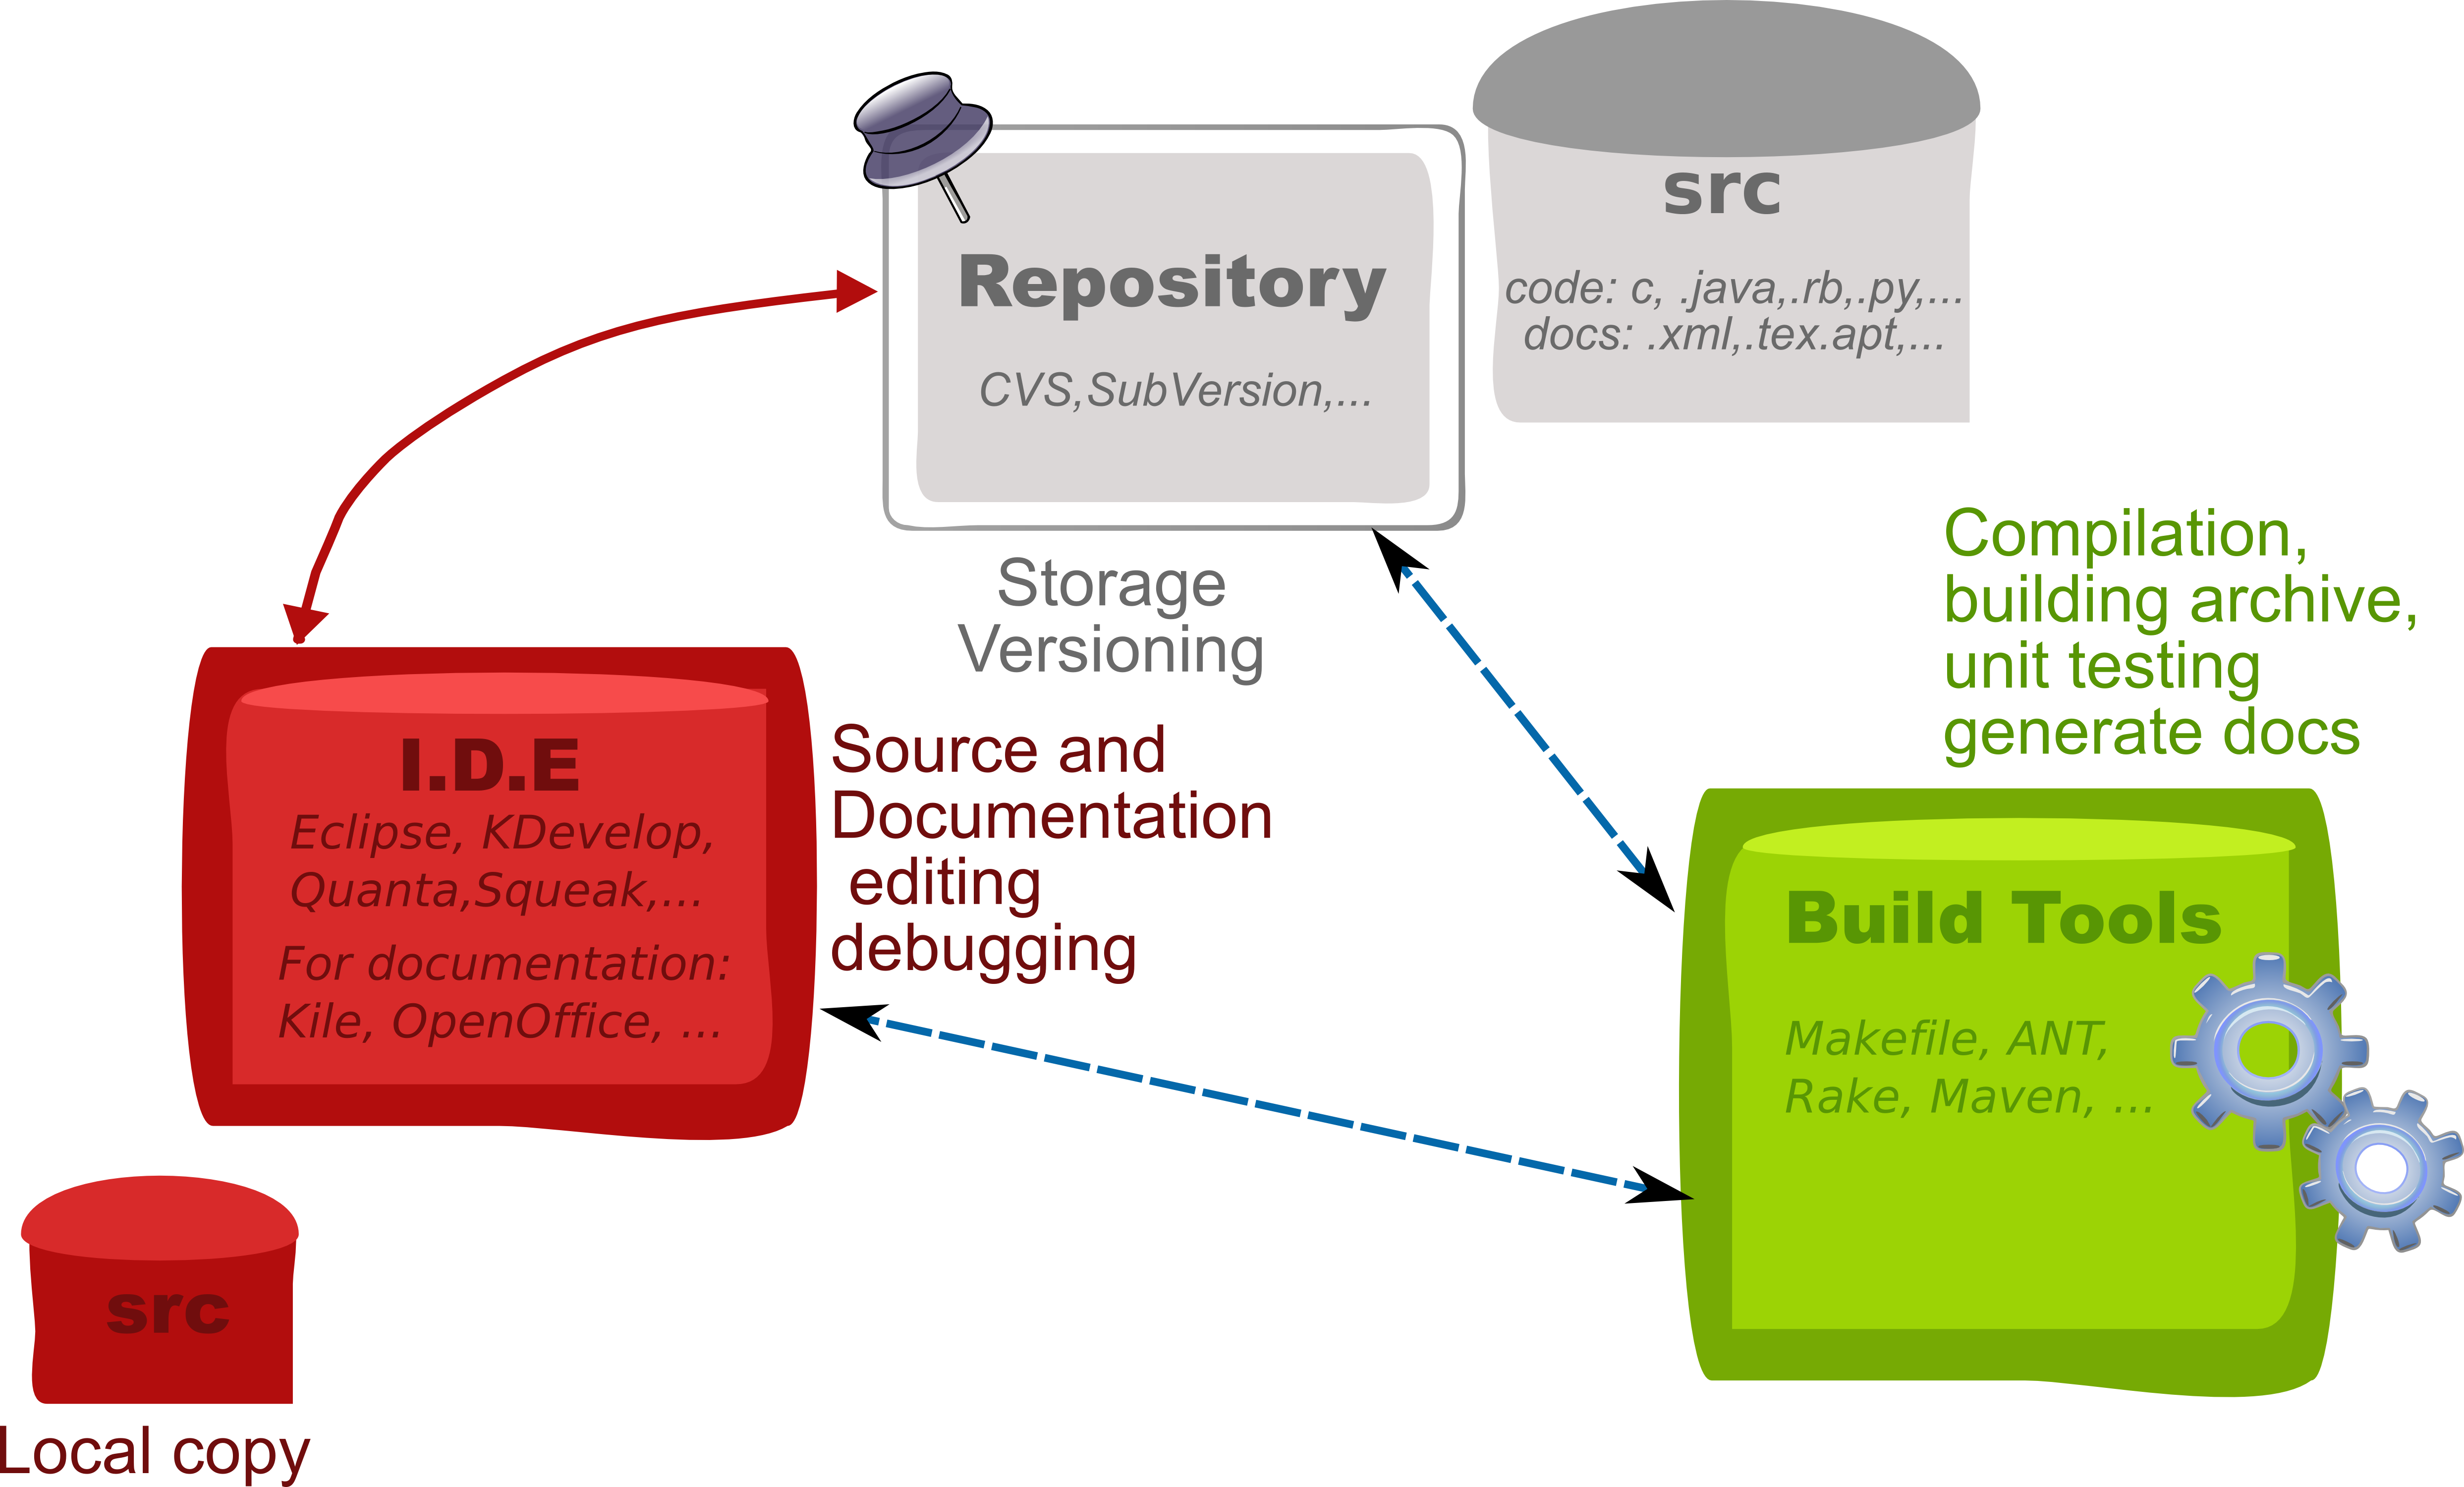
\includegraphics[scale=0.5]{../img/project-tools.png}
	\end{figure}
\end{frame}

\section{Outils de construction}
\subsection{Quel outil prendre et dans quel but ?}
\begin{frame}
 	\begin{block}{Objectif}
		\begin{itemize}
			\item Automatiser les tâches redondantes du projet:
				\begin{itemize}
					\item Exécution des tests unitaires
					\item Génération de la documentation
					\item ...
				\end{itemize}
			\item Permettre de facilement 'construire' le projet
			\item Externaliser les paramètres (adresse IPs, paramètres par défaut,...)
			\item Automatiser les déploiements (serveur de prod, pre-production)	
		\end{itemize}
	\end{block}
	\begin{block}{Le nerf du projet : le build}
	 	Le \textbf{build} est donc un \underline{point essentiel du projet} car
		il est le seul garant de sa \textbf{maintenabilité}.
		\textit{Un projet sans build peut être impossible à reprendre.}
	\end{block}
\end{frame}

\begin{frame}
 	\begin{block}{La relation technologie/build}
 	\end{block}
	\begin{columns}
		\column{.4\textwidth}
		\begin{block}{Ant}
			\begin{itemize}
				\item \textbf{Ant} est un outil de build Java pour Java et J2EE 
				\item \textbf{N-Ant} est Ant for C{\#} et .Net
			\end{itemize}
		\end{block}
		\column{.6\textwidth}
		\begin{figure}[hbtp]
			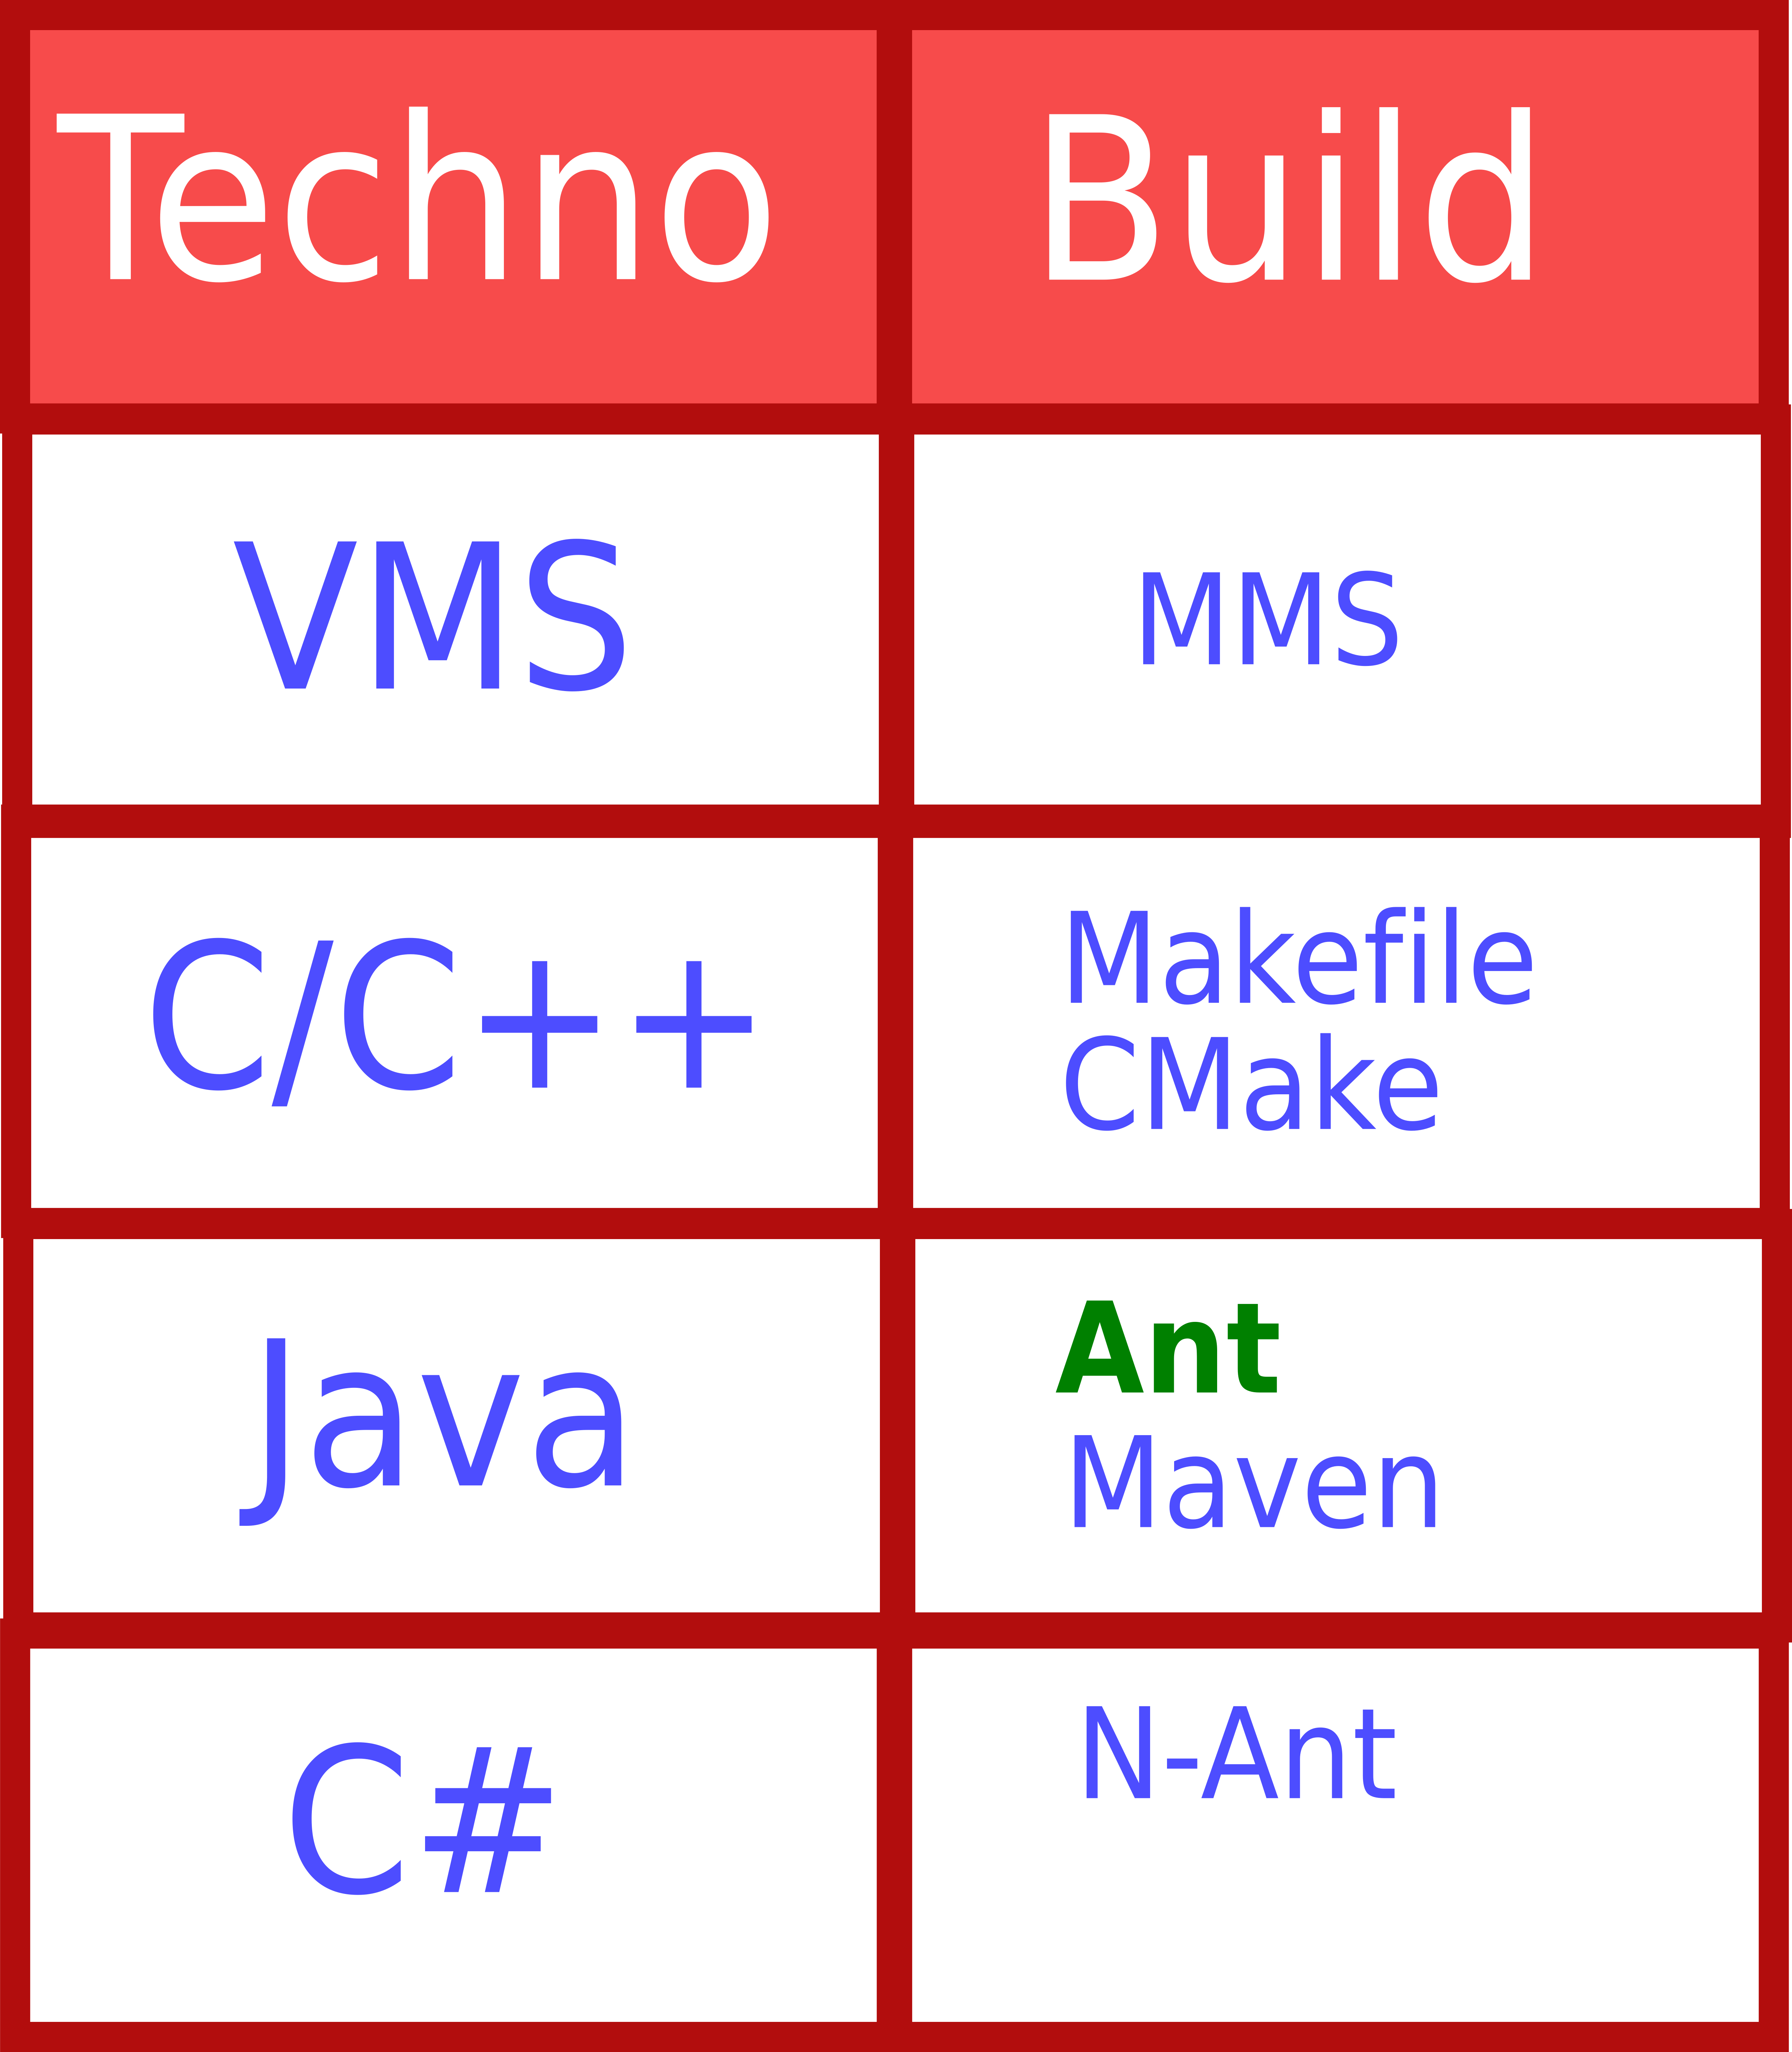
\includegraphics[scale=0.3]{../img/techno-build.png}
		\end{figure}
	\end{columns}
\end{frame}
\subsection{Ant}
\subsubsection{Concept clé de ant}
\begin{frame}
	\begin{block}{Histoire de Ant}
		\begin{itemize}
			\item Outil de \underline{Build en Java}, alternative à Makefile:
				\begin{itemize}
				 	\item Trop complexe
					\item Peu adapté à Java
				\end{itemize}
			\item Fichier de description de tâche en XML
			\item Conçu en Java, donc portable sur tout les OS
			\item Appel : \texttt{ant} + série de tâches ( ex: \texttt{ant clean compile install} )
		\end{itemize}
	 \end{block}
\end{frame}

\subsubsection{Structure du fichier}

\begin{frame}
	\begin{block}{Structure du fichier}
		\begin{itemize}
			\item Définit une série de tâche
			\item Définit dépendance entre les tâches
		\end{itemize}
		\lstinputlisting{../examples/syntax.xml}
	\end{block}
\end{frame}
\subsubsection{Fonctionnement}
\begin{frame}
  	\begin{block}{Ligne de commande}
		\begin{enumerate}
			\item Télécharger Ant et dézipper Ant
			\item Définir la variable ANT\_HOME qui contiendra l'adresse du répertoire Ant
			\item Ajouter dans le PATH 
			\begin{itemize}
 				\item Windows:\%ANT \textunderscore HOME\% \textbackslash bin
				\item Unix et Linux:\textdollar \textbraceleft ANT \textunderscore HOME\textbraceright /bin:\textbraceleft PATH\textbraceright
			\end{itemize}
			\item La commande \texttt{ant} sera désormais reconnue.
		\end{enumerate}
  	\end{block}

 	\begin{block}{Au sein d'Eclipse}
 	 	\textit{Etudiez après en TD...}
 	\end{block}
\end{frame}

\subsubsection{Syntax}
\begin{frame}
	\begin{block}{Définir des propriétés}
		\begin{itemize}
			\item Variables remplacées à l'exécution du script par leur valeur
			\item Externalisation de paramètres ( numéro de version, adresse ip,...)
			\item Définir une valeur à un seul endroit
		\end{itemize}
		\lstinputlisting{../examples/properties.xml}
	\end{block}
%	\begin{block}{Exemple d'exécution}
% \$ ant -f properties.xml\\
% Buildfile: properties.xml\\
% \\
% echo-properties:\\
%      [echo] Current project version is : 1.0\\
%      [echo] Source directory is : src\\
%      [echo] Build directory is : build\\
% \\
% BUILD SUCCESSFUL\\
% Total time: 0 seconds\\
%	\end{block}
\end{frame}

\subsubsection{Tâches les plus courantes}

\begin{frame}
\begin{block}{Ant task}
 	Il existe de nombreuses tâches associées aux actions:
	\begin{itemize}
		\item \textbf{echo}, pour afficher du texte
		\item \textbf{mkdir}, pour créer des répertoires
		\item \textbf{delete}, pour effacer des fichiers ou des répertoires
		\item \textbf{javac}, pour compiler du code java
		\item \textbf{javadoc}, pour générer la documentation à partir des commentaires javadoc
		\item \textbf{jar}, pour fabriquer un jar à partir de classes
		\item ...
	\end{itemize}
 	Liste complète : http://ant.apache.org/manual/coretasklist.html
\end{block}
\end{frame}
\subsubsection{TD:Utilisation au sein d'Eclipse}
\begin{frame}

	\begin{block}{Mise en place}
	 	\begin{itemize}
	 		\item Récupérer le projet 'tpbuild'
			\item Dézippez le, et placez le répertoire 'tpbuild' dans le workspace d'Eclipse
			\item Avec Eclipse, faite \textit{Fichier \textgreater Nouveau Projet- \textgreater Java Project}
			\item Appeler le projet comme le répertoire présent dans le workspace, soit 'tpbuild'
			\item Eclipse reconnaît la présence d'un projet existant. Valider.
	 	\end{itemize}
	\end{block}
\end{frame}

\begin{frame}
	\begin{block}{Utilisation de Ant}
		\begin{itemize}
			\item Dans le menu \textit{Fenêtres}, sélectioner l'option \textit{Vue}, et choisissez la vue \textit{Ant}
			\item Dans la fenêtre qui apparaît, sélectionnez le premier bouton \textit{Add build files}
			\item Sélectionner le fichier \textit{build.xml} déjà présent dans le répertoire 'tpbuild'
		\end{itemize}
	\end{block}

	\begin{block}{Conception du build}
	 	Ouvrez le fichier \textbf{build.xml} avec l'éditeur Ant de Eclipse et commencer par le \textbf{TODO FIRST}.
	\end{block} 
\end{frame}

\subsection{Pour aller plus loin... Maven}
\begin{frame}
	\begin{block}{Maven 2}
		\begin{itemize}
			\item Gestion automatique des dépendances
			\item Intégration avec le SCM
			\item Architecture évolutif à base de plugin
		\end{itemize}
		\begin{center}
			\textbf{Pour les projets de dernière année en Java, à considérer très sérieusement ! http://maven.apache.org/}
		\end{center}
	\end{block}
\end{frame}

%TODO: bonne pratique avec Ant

\section{Gestionnaire de sources}
\subsection{Les fonctionnalités des SCM}
\begin{frame}
	\begin{block}{SCM}
		\texttt{S}ource \texttt{C}onfiguration \texttt{M}anagement:
		\begin{itemize}
			\item Centraliser les sources
			\item Versionner les fichiers
			\item Travail concurrent, 2 philosophies
				\begin{itemize}
					\item lock 
					\item merge 
				\end{itemize}
			\item Tagger une version 
		\end{itemize}
	\end{block}
\end{frame}
\subsection{Lexique}
\begin{frame}
	\begin{block}{Lexique}
		\begin{itemize}
			\item checkout - récupérer une copie local du projet
			\item commit - appliquer ses modifications sur le projet
			\item diff - Etudier les différences entre 2 versions
			\item update - mettre à jour son projet local
			\item patch - proposer une modification, sans l'appliquer
			\item override \& commit - comitter de 'force' (attention !)
			\item override \& update - remplacer les copies locales modifié par celle du scm 
		\end{itemize}
	\end{block}
\end{frame}
\subsection{Les produits et l'avenir}
\begin{frame}
	\begin{block}{Etat de l'existant}
		\begin{itemize}
			\item Solutions libres comme CVS de plus en plus remplacé par SVN
			\item Solutions propriétaires multiples ( ClearCase,SourceSafe)
		\end{itemize}
	\end{block}
	\begin{block}{Pour aller plus loin}
		\begin{itemize}
			\item Les Forges
			\item L'intégration continue
		\end{itemize}
	\end{block}
\end{frame}
\subsection{TD:Utilisation de CVS avec Eclipse}
\begin{frame}
	\begin{block}{Enoncé}
		Avec le plugin CVS de Eclipse ou TortoiseCVS, réalisez les actions suivantes:
		\begin{enumerate}
			\item \textbf{Import} du projet fourni dans votre espace projet
			\begin{itemize}
				\item Attention à ne pas importer des fichiers binaires ou des artefacts !
			\end{itemize}
			\item Faire un \textbf{checkout} du projet, modifier un source puis utiliser \textit{Synchronize with Repository}
			\item Réaliser un patch avec \textbf{Create Patch} et étudier le fichier généré
			\item \textbf{commiter} le source modifié
			\item Faites un \textbf{update} du projet pour prendre en compte mes modifications
		\end{enumerate}
	\end{block}
\end{frame}
\section{Fin}
\begin{frame}
	\begin{block}{Latex}
		Ce slideware a été réalisé à l'aide du package \textbf{beamer} pour 
		\begin{center}
			
\includegraphics[scale=0.3]{../img/latex.png}
			% latex.png: 282x140 pixel, 95dpi, 7.54x3.74 cm, bb=0 0 214 106
		\end{center}
	\end{block}

	\begin{block}{Licence associée}
		Cette présentation et son contenu est placé sous licence Creative Commons, vous pouvez réutiliser cette dernière en respectant les clause suivantes:
		\begin{itemize}
			\item \textbf{Paternité}: Citer le nom de l'auteur original.
			\item \textbf{Pas d'Utilisation Commerciale}: Vous n'avez pas le droit d'utiliser cette présentation à des fins commerciales.
		\end{itemize}
	\end{block}
\end{frame}

% TODO
% \section{Annexes}
% \begin{frame}
% 	\begin{block}{Comparaison avec un fichier Makefile}
% 		\lstset{
% 		language=csh, 
% 		backgroundcolor=\color{white}, 
% 		basicstyle=\small, 
% 		showstringspaces=false,
% 		stringstyle=\ttfamily,
% 		commentstyle=\color{vert_commentaire},
% 		keywordstyle=\color{blue}\bfseries\emph
% 		}
% 		\lstinputlisting{../examples/Makefile}
% 	\end{block}
% \end{frame}


\end{document}